Note that composite particles can look like (fundamental) point particles under certain circumstances. Basically this has to do if the distance resolution (directly related to the energy of the interactions considered through $\lambda = h/p$) is such that the structure of the particle can be resolved. Electrons moving around an atomic nucleus have energies of a few tens of $eV$ and a wavelength similar to the size of an atom ($\sim 10^{-10}$m), much larger than the nucleus with $~10^{-10}$m, and from that point of view, the nucleus looks like a point particle. At somewhat larger energies/shorter wavelengths, nuclear structure of protons and neutrons becomes apparent, and att HERA, electrons collided with protons at energies where they could even resolve the proton structure. It is therefore in principle possible that the particles we now consider fundamental are in fact composites particles that would reveal their composite structure only at far higher energies.


\subsection{Notation}
 We will label our co-ordinates with indices from 0 to 3, where 0 is the
 time component, and 1-3 the space components 
\[ (x^0, x^1, x^2, x^3) = (ct, x, y, z)\]
%  
  The $x$ without an arrow on top represents the entire 4-vector:
\[
 x = (x^0, x^1, x^2, x^3)
\]
  while $\vec{x}$ represents the space components only:
\[
\vec{x} = (x^1, x^2, x^3) = (x, y, z)
\]
Four-vectors are defined as objects that transform under Lorentz transformations like  $(c\mathit{\Delta t}, \mathit{\Delta x}, \mathit{\Delta y}, \mathit{\Delta z})$, i.e. differences in $ct, x, y, z$. If we exclude shifts of the coordinate system, and only allow boosts and rotations (i.e. proper Lorentz transformations), then $(ct, x, y, z)$ transforms exactly like $(c\mathit{\Delta t}, \mathit{\Delta x}, \mathit{\Delta y}, \mathit{\Delta z})$. The most important four-vectors are:
\begin{align}
  \Delta x &= \vIV{c\Delta t}{\Delta x}{\Delta y}{\Delta z}
& p &= \vIV{E/c}{p_x}{p_y}{p_z}
& \partial &= \vIV{\partdbyd{}{(ct)}}{-\partdbyd{}{x}}{-\partdbyd{}{y}}{-\partdbyd{}{z}}
\end{align}



\subsection{Summary of B mixing}
\label{sec:BMixSummary}
\begin{itemize}
 \item \Bdo\ and \Bdob\ are the so-called flavour eigenstates. They
 have well-defined flavour content (i.e. one $\bar{b}$ and one $d$, or
 one $b$ and one $\bar{d}$ respectively. These are the states produced
 in strong interactions.
 \item The states with well-defined mass and lifetime are however \Bh\
 and \Bl\ (``B-heavy and B-light''). They are superpositions of \Bdo\
 and \Bdob:
\begin{equation}
\label{eq:th.a.def_Bl_Bh_2}
\ket{\prt{B_{H,L}}} = p \ket{\Bo} \mp q \ket{\Bob},
\end{equation}
with $|p|^2 + |q|^2 = 1$ and 
  \item The most important parameters that describe this system are
 $\Delta m$ the mass difference between \Bh\ and \Bl, and
 $\Delta\Gamma$, the width (= inverse lifetime, $\Gamma = 1/\tau$)
 difference of \Bh\ and \Bl.
 \item \Bh\ and \Bl\ represent the 'physical' B states. They travel
 through space and time happily and independently - once a \Bh\ always
 a \Bh, once a \Bl, always a \Bl.
  \item However, \Bo\ and \Bob\ continuously transform into each other
  as they travel through space and time. They oscillate between being
  a \Bo\ and a \Bob\ with a frequency that is given by the mass
  difference between \Bh\ and \Bl, $\Delta m$.
A particle that is born as a \Bo\ has the probability of being
  detected as a \Bob\ of:
\begin{equation}
\left| \braket{\Bob}{\Bo}(t) \right|^2 = e^{-\Gamma t} \left(1 - \cos
(\Delta m t)\right)
\end{equation}
 where $t$ is the decay time in the restframe of the \Bo. $\Gamma$ is
 the average lifetime of \Bh, \Bl\ - we made the approximation that
 $\Delta\Gamma$ is negligible, which is OK for \Bdo\ and OK-ish for
 \Bso. The exponential represents the
 usual decay law. The $\cos \Delta m t$ term represents the
 oscillation.
\end{itemize}




 If $\exp\left(-i\op{H}\right)$ were a unitary matrix, the ``length''
 of the state vector (i.e. the probability density), would remain
 constant. This would be the case if $\op{H}$ were Hermitian, and this
 is what we would normally expect for a \Se\ that describes the
 complete set of possible states.
 
 However, this is the \Se\ restricted to the $\ket{\Bo}-\ket{\Bob}$
 subspace of state vectors. The system is allowed to leave the
 $\ket{\Bo}-\ket{\Bob}$ subspace by decaying to other particles,
 hence $\mathbf{H}$ in equation \ref{eq:th.a.se} will not be
 Hermitian.

 A general matrix \op{H} can be expressed in term of the Hermitian
 matrices $\op{M}$ and $\op{\Gamma}$ as
\begin{equation}
 \op{H} = \op{M} - \frac{i}{2} \op{\Gamma}
\end{equation}
 Where the Hermitian part $\op{M}$ represents the energy (mass) of the
 system, while the non-Hermitian part $\frac{i}{2} \op{\Gamma}$ the
 decay to other states.


\subsection{A closer look at B mixing and CP Violation*}
\label{sec:details}
The \Se\ for a superposition of flavour eigenstates, $ a \ket{\Bo} + b
\ket{\Bob}$, is:
\begin{equation}
\label{eq:th.a.se}
%
i\dbyd{}{t}\vII{a}{b}= \op{H} \vII{a}{b}.
%
\end{equation}\\
 The solution can formally be written down as
\begin{equation}
 \vII{a(t)}{b(t)} = \exp\left(-i\op{H}\right) \vII{a(0)}{b(0)}
\end{equation}
 If $\exp\left(-i\op{H}\right)$ were a unitary matrix, the ``length''
 of the state vector (i.e. the probability density), would remain
 constant. This would be the case if $\op{H}$ were Hermitian, and this
 is what we would normally expect for a \Se\ that describes the
 complete set of possible states.
 
 However, this is the \Se\ restricted to the $\ket{\Bo}-\ket{\Bob}$
 subspace of state vectors. The system is allowed to leave the
 $\ket{\Bo}-\ket{\Bob}$ subspace by decaying to other particles,
 hence $\mathbf{H}$ in equation \ref{eq:th.a.se} will not be
 Hermitian.

 A general matrix \op{H} can be expressed in term of the Hermitian
 matrices $\op{M}$ and $\op{\Gamma}$ as
\begin{equation}
 \op{H} = \op{M} - \frac{i}{2} \op{\Gamma}
\end{equation}
 Where the Hermitian part $\op{M}$ represents the energy (mass) of the
 system, while the non-Hermitian part $\frac{i}{2} \op{\Gamma}$ the
 decay to other states.

 It can be shown that \cpt\ invariance implies
 

%%
\begin{equation}
\bra{\Bo}\op{H}\ket{\Bo} = \bra{\Bob}\op{H}\ket{\Bob}.
\end{equation}\\
 Therefore the diagonal elements of \op{H} are the same and \op{H} can
 be written as:
\begin{equation}
\op{H}=\mII{h_{11}}{h_{12}}{h_{21}}{h_{11}}.
\end{equation}
 As \op{M} and \op{\Gamma} are Hermitian, their off-diagonal elements
 are complex conjugates of each other:
\begin{equation}
\op{M}=\mII{m_{11}}{m_{12}}{m_{12}^*}{m_{11}}
,\;\;
\op{\Gamma}=\mII{\Gamma_{11}}{\Gamma_{12}}{\Gamma_{12}^*}{\Gamma_{11}}.
\end{equation}\\
 \op{H} has the following eigenvalues:
\begin{equation}
\lambda_{H,L}=h_{11}\pm \sqrt{h_{21}\cdot h_{12}}
\end{equation}
 and eigenvectors
\begin{equation}
\vec{v}_{H,L}\equiv\vII{p}{\mp q}
\end{equation}
 with 
\begin{equation}
\frac{q}{p}= -\sqrt{\frac{h_{21}}{h_{12}}}.
\end{equation}\\
 The diagonalised Hamiltonian \op{H_d} is:
{\small
\begin{eqnarray}
%
\lefteqn{\op{H_d} = \mII{H_H}{0}{0}{H_L} }\nonumber\\
         & &
= \mII{h_{11} + \sqrt{h_{12} h_{21}}\!\!\!}{0}
    {0}{\!\!\!h_{11} - \sqrt{h_{12} h_{21}}}
.
\nonumber\\
\mbox{}
\end{eqnarray}}\\
 The diagonal mass and decay matrices, defined by
\begin{equation}
\op{M_d}=\frac{1}{2}\left(\op{H_d}+\op{H^{\dagger}_d}\right), \;\;
\op{\Gamma_d}=i\left(\op{H_d} - \op{H^{\dagger}_d}\right)
,
\end{equation}
 are:
\begin{eqnarray}
\op{M_d}&=&\mII{M_H}{0}{0}{M_L} \nonumber\\
        &=&\mII{\Real\!\left(H_H\right)}{0}{0}{\Real\!\left(H_L\right)}\\
\op{\Gamma_d}&=&\mII{\Gamma_H}{0}{0}{\Gamma_L} \nonumber\\
             &=&\mII{-2\Imag\!\left(H_H\right)}{0}{0}{-2\Imag\!\left(H_L\right)}
.
\nonumber\\
\mbox{}
\end{eqnarray}
\\
 The subscripts L and H stand for the ``light'' and the ``heavy''
 physical \Bo-states. The mass- and width difference between those
 states is:
\begin{equation}
\Delta\!m = M_H-M_L, \;\;\;
\Delta\!\Gamma=\Gamma_H-\Gamma_L
\end{equation}\\
which are related to $m_{ij}$ and $\Gamma_{ij}$ via
{\small
\begin{eqnarray}
\lefteqn{\Delta\!m - \frac{i}{2}\Delta\!\Gamma =2\sqrt{h_{12} h_{21}}} 
\nonumber \\
&=&
2\sqrt{\left(m_{12}-\frac{i}{2}\Gamma_{12}\right)
\left(m^*_{12}-\frac{i}{2}\Gamma^*_{12}\right)} 
,
\nonumber \\
\mbox{}
\end{eqnarray}
}\\
giving:
\begin{equation}
\left(\Delta\!m\right)^2 - \frac{1}{4}\left(\Delta\!\Gamma\right)^2
 = 
 4 \left|M_{12}\right|^2 - \left|\Gamma_{12}\right|^2,
\end{equation}\\
\begin{equation}
\Delta\!m \Delta\!\Gamma
 = 4\Real\!\left(M_{12}\Gamma^*_{12}\right)
\end{equation}\\
and
\begin{eqnarray}
\label{eq:th.a.qbypis}
\frac{q}{p}&=&-\sqrt{\frac{h_{21}}{h_{12}}} =
-\frac{\sqrt{h_{12}h_{21}}}{h_{12}} \nonumber\\
&=& -\frac{ \frac{1}{2}\left(\Delta\!m - \frac{i}{2}\Delta\!\Gamma
\right) }{m_{12} - \frac{i}{2} \Gamma_{12}}\nonumber\\
&=& -\frac{m^*_{12} - \frac{i}{2} \Gamma^*_{12}}{
\frac{1}{2}\left(\Delta\!m - \frac{i}{2}\Delta\!\Gamma
\right) }
.
\end{eqnarray}

subsubsection{\cp\ Violation in the Mixing}
\label{sec:th.a.cpinmixing}
 Using a phase convention in which
\begin{equation}
\cp \ket{\Bo} = \ket{\Bob},
\end{equation}\\
 the \cp\ operator in \Bo--\Bob\ space is given by the first Pauli spin
 matrix:
\begin{equation}
\cp = \sigma^1 = \mII{ 0 }{ 1 }{
                       1 }{ 0 }
.
\end{equation}\\
 We can write the Hamiltonian, like any other $2\times 2$ matrix, as
\begin{equation}
\op{H} = a^0 \mathbf{1} + a^1 \sigma^1 + a^2 \sigma^2 + a^3 \sigma^3
\end{equation}\\
where $a^i$ are four complex numbers. Then \cp\ invariance requires:
\begin{equation}
\left[H_{\mathrm{\cp-conserving}},\sigma^1\right] = 0
.
\end{equation}
With the above definitions:
\begin{equation}
\left[H,\sigma^1\right] = - a^2 \sigma^3 +  a^3 \sigma^2
.
\end{equation}\\
Therefore, for a \cp\ conserving Hamiltonian, $a^2 = a^3 = 0$, and the
most general \cp\ conserving Hamiltonian can be written as:
\begin{equation}
\op{H}_{\mathrm{\cp-conserving}} = \mII{  a^0  }{  a^1  }{
                                          a^1  }{  a^0  }
.
\end{equation}\\
With equation \ref{eq:th.a.qbypis} we get therefore:
\begin{equation}
\mbox{ \cp\ Conservation} \Rightarrow p = -q
\end{equation}\\
 Changing to a general phase convention with
$\cp \ket{\Bo} = e^{i\alpha} \ket{\Bob}$
 is equivalent to a basis transformation:
\begin{equation}
\ket{\Bdo}^{\prime} = e^{+i\alpha/2}\ket{\Bdo},\;\;\;
\ket{\Bdob}^{\prime} = e^{-i\alpha/2}\ket{\Bdob}
.
\end{equation}\\
The column-vectors transform like:
\begin{equation}
\vII{a}{b}^{\prime} = 
\mII{ e^{-i\alpha/2} }{ 0 }{ 0 }{ e^{ i\alpha/2} }
\vII{a}{b}
,
\end{equation}\\
and \cp\ is given by:\\
{\footnotesize
\begin{eqnarray}
&& \mII{ e^{-\frac{i}{2}\alpha} }{ 0 }{ 0 }{ e^{ \frac{i}{2}\alpha} }
        \mII{     0         }{ 1 }{ 1 }{        0        }
        \mII{ e^{\frac{i}{2}\alpha}}{ 0 }{ 0 }{ e^{
        -\frac{i}{2}\alpha}  }
\nonumber\\
   &=&  \mII{ 0 }{e^{-i\alpha}   }{ e^{ i\alpha}   }{0}
.
\end{eqnarray}}\\
Therefore 
\begin{equation}
\cp \ket{\Bo} = e^{i\alpha}\ket{\Bob}
\end{equation}\\
as required. In this basis, \op{H} is given
by:\\
\begin{equation}
\op{H}=
 \mII{ h_{11}             }{  h_{12} e^{-i\alpha} }{
       h_{21} e^{i\alpha} }{  h_{11}              }
\end{equation}\\
and the ratio $q/p$ transforms like:
\begin{equation}
\frac{q}{p} \to \frac{q}{p} e^{i\alpha}
.
\end{equation}\\
So the phase--convention independent statement is:
\begin{equation}
\label{eq:th.a.qpmixing}
\mbox{ \cp\ Conservation} \Rightarrow \mod{p}=\mod{q}
\end{equation}\\

\subsection{Important aspects of Feynman diagrams (brief reminder)}

-- Time runs from left to right in the sense that:
\begin{itemize}
\item LHS of the diagram is the initial state
\item RHS of the diagram is the final state
\item Middle of the diagram is how it happened
\end{itemize}

-- Anti-particle arrows should point in negative time direction, for example for the $e^+e^-\to \mu^+\mu^-$ process we have
\begin{center}
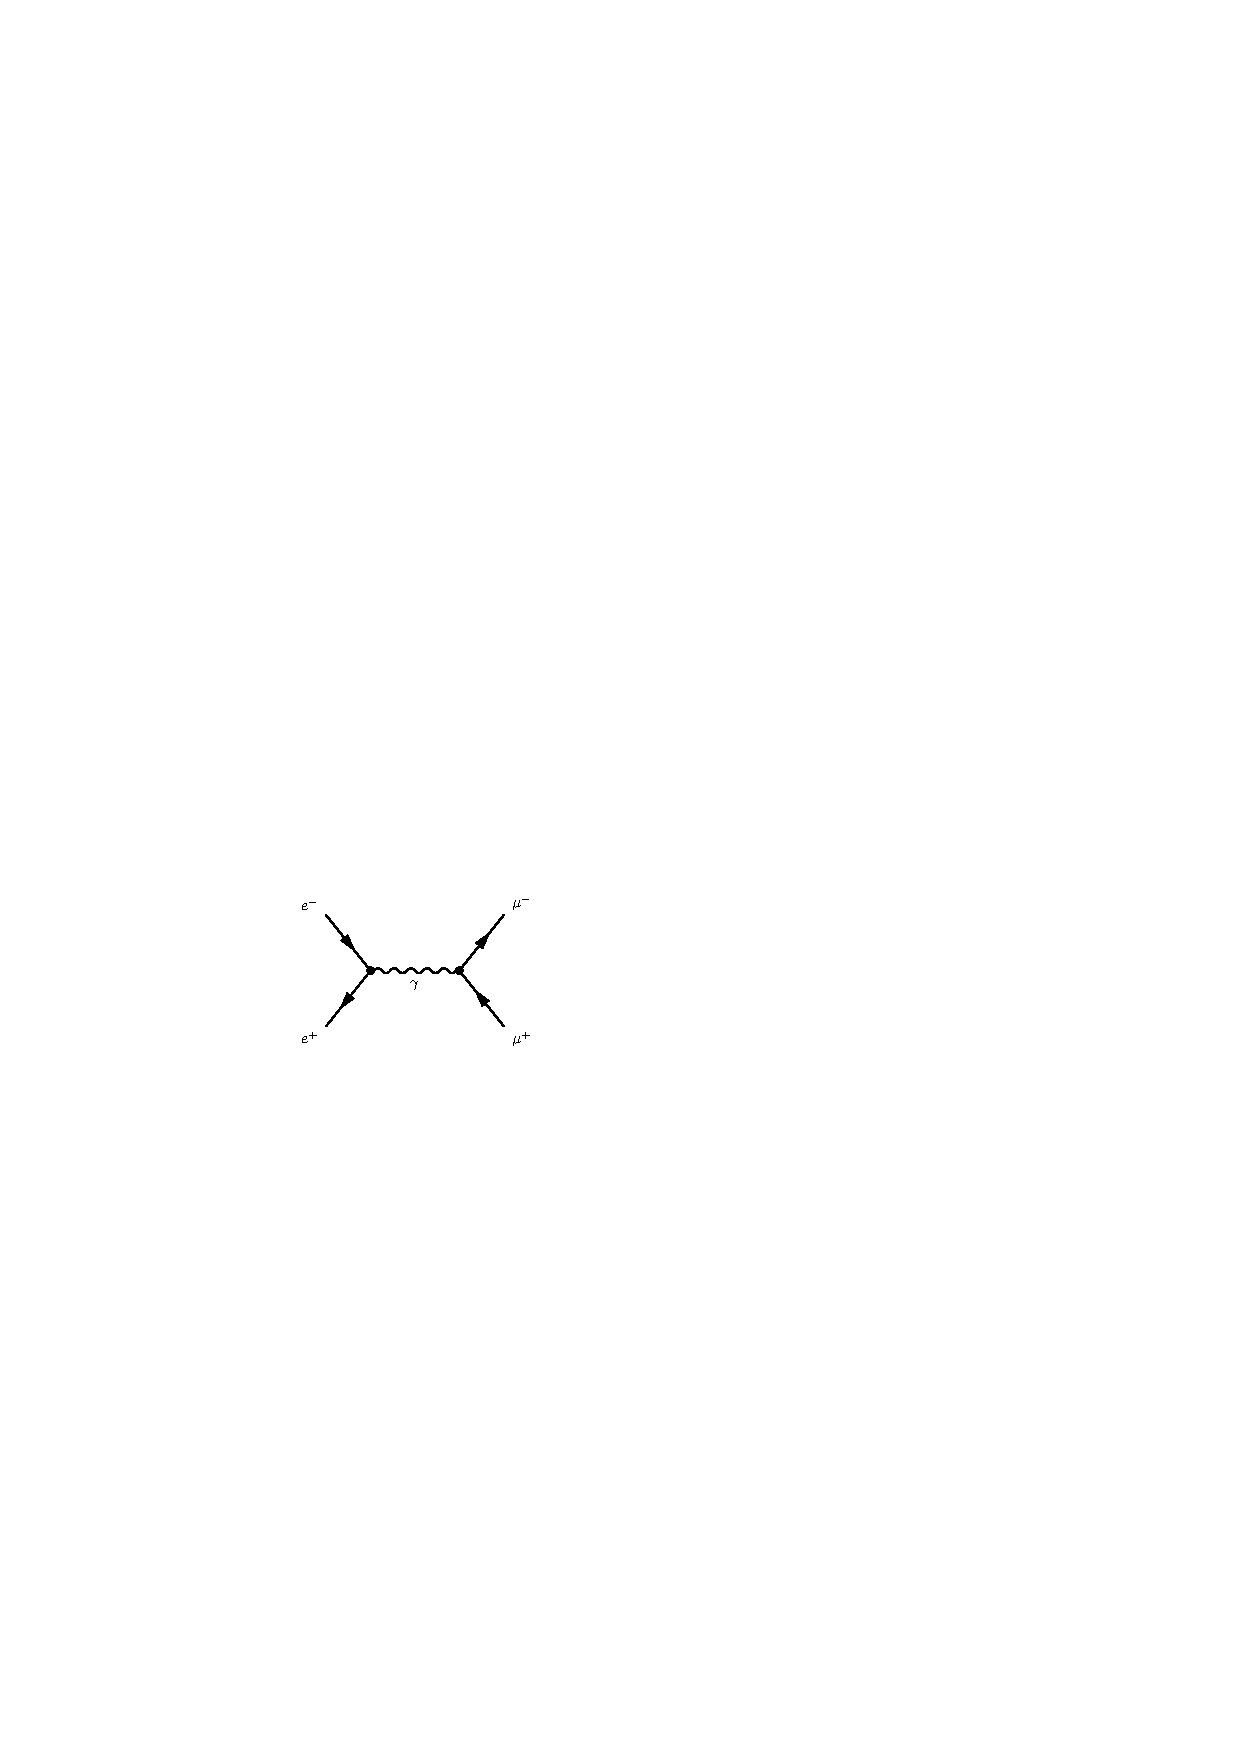
\includegraphics[width=0.5\textwidth]{fig/forcerange/eetomm.pdf}
\end{center}


-- The intermediate particle in Feynman diagrams is considered virtual in the sense that 
$E^2\neq p^2+m^{2}$. The intermediate particle is said to be ``off-shell''. In the example shown below the intermediate particle is the photon and $E^2_{\gamma}\neq p^2_{\gamma}+m_{\gamma}^{2}$ (where $m_\gamma=0$). 
\begin{center}
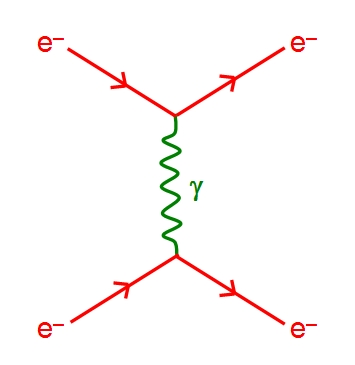
\includegraphics[width=0.5\textwidth]{fig/forcerange/qed.jpg}
\end{center}

-- Each vertex contributes a coupling strength factor $g^2$ to the probability of the process to occur. In EM interactions $g^2$ is related to the fine structure constant $\alpha_{\rm EM}=\frac{1}{137}$. So for the example above, the process occurs at a rate proportional to $\alpha_{\rm EM}^2$\footnote{In fact as you will see later and next year there are additional factors that affect the overall rate}.



-- At each vertex energy and momentum are conserved however we cannot have
diagrams with a single vertex. That is because diagrams of the form below 
\begin{center}
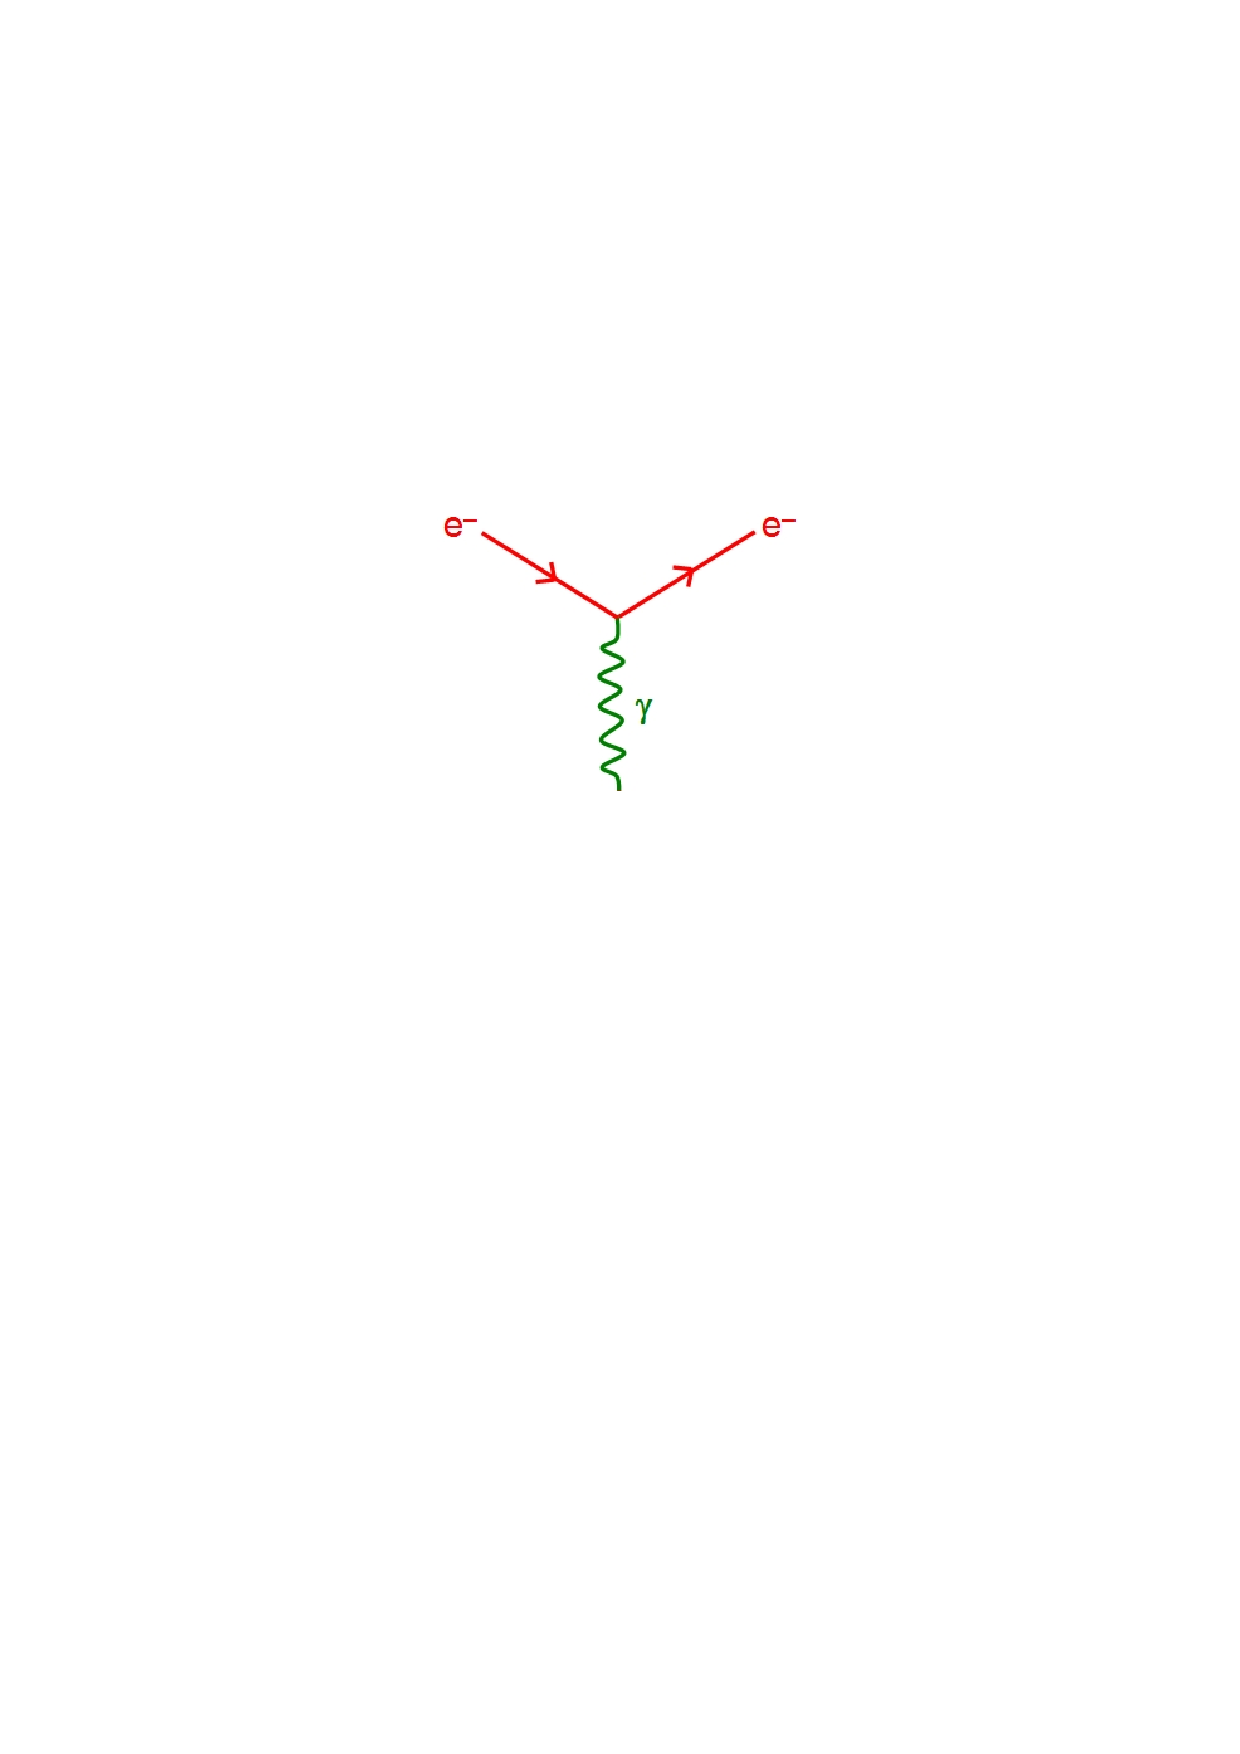
\includegraphics[width=0.45\textwidth]{fig/forcerange/qed_half.pdf}
\end{center}
violate energy conservation.\\


\exercise{ Show the diagram above violates energy
conservation. In this case the photon is real ie not virtual.}





%%
\section*{Natural Units}
To "ease you in" to the course a bit, we kept factors of $\hbar$ and $c$. However, it is time to become a proper particle physicist, use (initially a bit unfamiliar, but eventually much easier) "natural units" with $c=\hbar=1$ as discussed in \secref{sec:naturalUnits}. It's worth it.

\section{Reminder: Cross section, decay rates, and Feynman Diagrams}
Some of this is already described in \secref{sec:DecaysAndReaction}, this is just to clarify some conventions and notations that we will need for the next few sections. Especially, this concerns the connection between Feynman diagrams, and decay rates, and reaction rates.

Let us consider first the decay of a particle $A$ to particles $B, C$. The probability of this process to take place can calculated as the product of two terms:
\begin{itemize}
\item Squared magnitude of the quantum mechanical (complex) amplitude for the transition $A\to B, C$, $\left|\mathcal{M}_{BC,A}\right|^2$. (For a generic initial state $i$ and final state $f$, we'll write $\mathcal{M}_{fi}$ instead of $\mathcal{M}_{BC,A}$.)
\item The density of $B, C$ momentum states that are available, called \emph{density of states}, \emph{phase space density}, or \emph{available phase space}, and often, lazily, simply \emph{phase space}. You might argue that there is exactly one momentum $\vec{p}_B = -\vec{p}_C$ that $B$ can have in the $A$ restframe, if we know the masses of $A, B, C$, but in reality there is always (however small) a range due to the uncertainty principle, so the number of final states, and hence the observed decay rate, is proportional to the density of states near $\vec{p}_B$. This turns out to be related to the energy release in the decay as stated in \secref{sec:DecaysAndReaction}, in such a way that the larger the energy release, the bigger the density of states. This is derived in the optional \secref{sec:densityOfStates} below.
\end{itemize}

For processes such as scattering $A, B \to C, D$, we also have to take into account "how hard I try" to shoot particles $A$ and $B$ into each other. This is expressed as the luminosity $\mathcal{L}$, measured in the number of particles impingining on each other per unit volume per unit time. In order to separate the running conditions of our experiment (expressed as $\mathcal{L}$) from the physics, we use the cross section $\sigma$, defined such that 
\begin{equation}
\mathrm{rate} = \mathcal{L} \cdot \sigma
\end{equation}

For the discussion that follows it is especially important to remember that\\
\fbox{\parbox{0.99\textwidth}{
\begin{itemize}
\item $\mathcal{M}_{fi}$ represents a quantum mechanical amplitude to go from one state $i$ to another $f$. It encapsulates "the physics". $\mathcal{M}_{fi}$ is what we calculate with Feynman diagrams. $\mathcal{M}_{fi}$ is a complex number. The rate is proportional to $\left|\mathcal{M}_{fi}\right|^2$. But the fact that $\mathcal{M}_{fi}$, and the Feynman diagrams that contribute to it, are complex, matters if several complex amplitudes interfere with each other. E.g. if $\mathcal{M}_{fi}^{\mathrm{total}} = A_1 e^{i\phi_1} + A_2 e^{i\phi_2}$ (where $A_i$, $\phi_i$ are real number and $A_1 e^{i\phi_1}$ might be represented by one Feynman diagram, and $A_2 e^{i\phi_2}$ by another), then $\left|\mathcal{M}_{fi}\right|^2 = A_1^2 + A_2^2 + 2A_1 A_2 \cos(\phi_2-\phi_1)$
\item The rate at which a process happens depends also on the density of states (proportional to the magnitude of the momentum squared), and, for scattering experiments, on the luminosity
\end{itemize}
}}

\fbox{\parbox{0.99\textwidth}{
\paragraph{Potential Convention Confusion}
Sometimes, typically in rough `order of magnitude' estimates, Feynman diagrams are evaluated directly for $\left|\mathcal{M}_{fi}\right|^2$, in which case one puts for QED processes an factor of $e^2$ or $ 2\pi \alpha $ for each vertex in the Feynman diagram. This is not what we will do. Our Feynman diagrams (from now on) will always be evaluated for $\mathcal{M}_{fi}$. QED diagrams will have a factor of $e$ or $\sqrt{2\pi \alpha}$ for each vertex. This is not only important for consistency, but also because we will come across complex vertex factors and interference effects, so adding up complex amplitudes \emph{before} squaring them to get a probability is crucial.
}}

\subsection{Golden Rules}
\begin{figure}
\centering
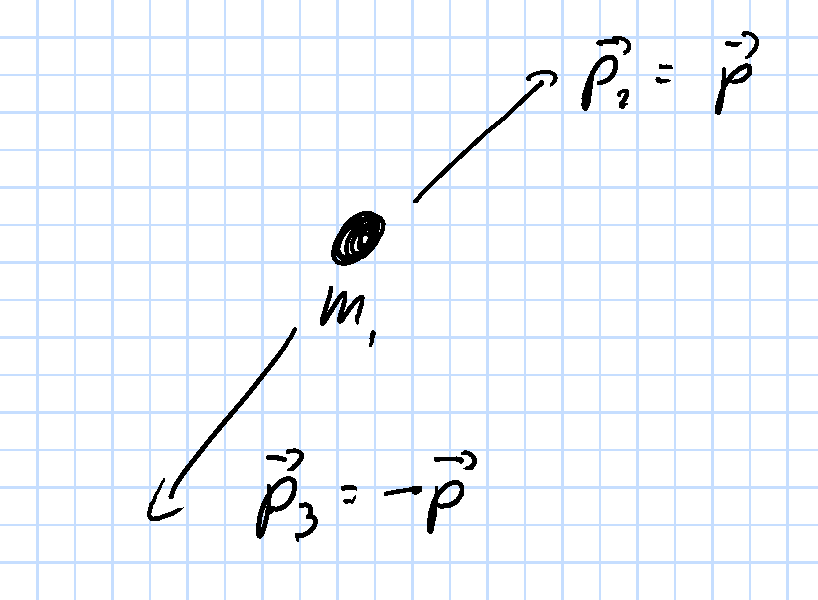
\includegraphics[width=0.4\textwidth]{fig/weak/Decay122}
\caption{Decay rate of particles $1$ into two particles (labelled $2$ and $3$) in the cm frame.\label{fig:Decay122}}
\end{figure}
\begin{figure}
\centering
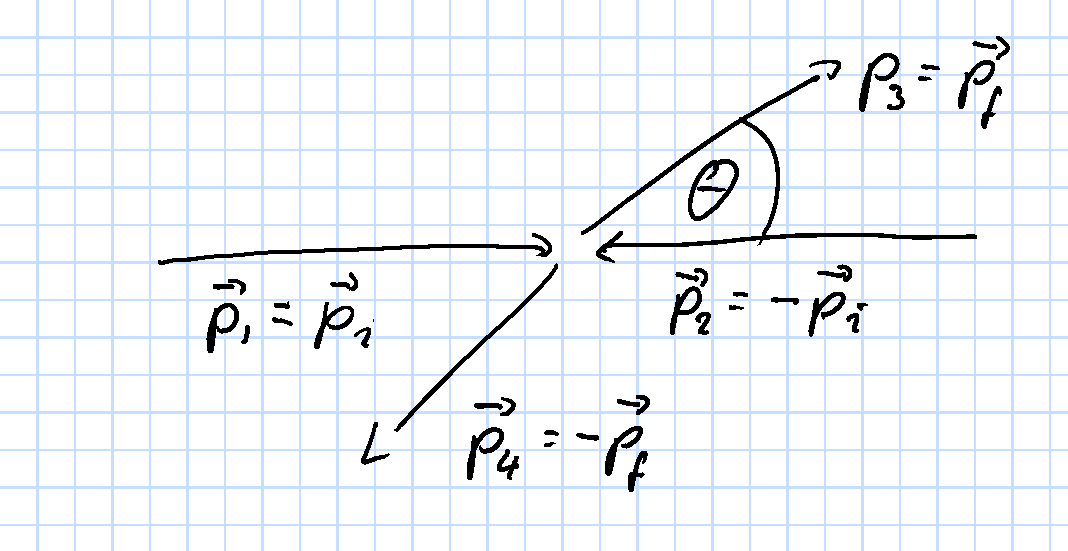
\includegraphics[width=0.7\textwidth]{fig/weak/ScatteringGeneric222}
\caption{$2$ particle to $2$ particle scattering, $1,2 \to 3,4$.\label{fig:ScatteringGeneric222}}
\end{figure}

These golden rules relate $\mathcal{M}_{fi}$ and hence the Feynman rules to measurable quantities, taking into account phase space density. 
\paragraph{Golden Rule Decay Rates in cm frame}
(see \figref{fig:Decay122})
Decay of particle $1$ to particles $2, 3$ in the cm frame 
\begin{equation}
\Gamma_k = \frac{S}{8\pi} \frac{|\vec{p}|}{m_1^2} \left|\mathcal{M}_{fi}\right|^2
\end{equation}
Where $m_1$ is the mass of the decaying particle, and $\vec{p}$ is momentum of one of the daughter particles, $\vec{p} = \vec{p}_2 = -\vec{p_3}$. The subscript $k$ in $\Gamma_k$ indicates that this is the \emph{partial} width for the decay to this particular final state (that we label $k$). $S$ is $1$ when the final state particles are distinguishable (as in \prt{\pi^+ \to \mu^+ \nu_{\mu}}), except when the two final state particles are identical (as in \prt{\pi^0 \to \gamma \gamma}), in which case $S = \half$.
This is what you can do with the result of this calculation:
\begin{itemize}
\item $\Gamma_k$ is the partial width of the decay of particle $1$ to particles $2, 3$.
\item If I add up all partial widths (i.e. $\Gamma_k$ calculated for all possible final states $k$, added together) I get the total width $\Gamma = \sum_k \Gamma_k$. Its inverse is the average lifetime of the particle, $\tau = 1/\Gamma$. If I start with $N_0$ particles, I expect, after time $t$ (in the particles' restframe), to find $N(t) = N_0 e^{-\Gamma t}$.
\item If we have $N$ particles, the rate at which they will decay to this given final state is $N\Gamma_k$ (note that $N$ will decrease exponentially with time, $N(t) = N_0 e^{-\Gamma t}$).
\item If I observe $n$ decays of this given type of particle, the fraction of decays $n_k$ that I expect to find in final state $k$ is $n_k/n = \Gamma_k/\Gamma$. This ratio is called the Branching Fraction.
\end{itemize}


\paragraph{Golden rule for scattering in CM frame}
This is for calculating the differential cross section for two particles in the CM frame, which have the momenta $\vec{p}_1 = \vec{p}_i$ and $\vec{p}_2 = -\vec{p}_i$, that scatter into two final state particles with momenta $\vec{p}_3 = \vec{p}_f$ and $\vec{p}_4 = -\vec{p}_f$ as illustrated in \figref{fig:ScatteringGeneric222}:
\begin{equation}
\frac{d \sigma}{d\Omega}= \frac{S}{64\pi^2} \frac{1}{(E_1 + E_2)^2} \frac{|\vec{p}_f|}{|\vec{p}_i|} \left|\mathcal{M}_{fi}\right|^2
\end{equation}
We label the incoming particles as $1, 2$ and the outgoing as $3, 4$.
Here, $d\Omega$ is a solid angle element $d\phi\; d(\cos\theta)$. The scattering angle $\theta$ is defined relative to $\vec{p}_i$, and $\phi$ (not shown in the diagram) is the angle of rotation around the axis defined by the initial momenta (you have a choice how you define these angles, e.g. is $\theta$ the angle of $\vec{p}_3$ relative to $\vec{p}_1$ or $\vec{p}_4$ relative to $\vec{p}_1$, that's why it's always good to draw  diagram to define this). So, $\mathcal{L} \cdot \frac{d \sigma}{d\Omega}$ is proportional to the number of events per unit time that we will observe where $\vec{p}_f$ is in the direction between $\phi$ and $\phi + d\phi$ and between $\cos(\theta)$ and $\cos(\theta) + d\cos(\theta)$ when we shoot initial state particles at each other with luminosity $\mathcal{L}$. The quantity $\frac{d \sigma}{d\Omega}$ is proportional to that, but independent of the luminosity. It is measured in units of $[\mathrm{area}]^2$, usually expressed in "barn", with symbol \units{b}. One barn is approximately the size of a nucleus: $\un{1}{b} = (\un{10^{-14}}{m})^2 = \un{100}{fm^2}$. A nucleus is huge in terms of particle physics cross sections, hence the term barn (as in "your aim is so poor, you couldn't hit the broad side of a barn"). Typical cross sections we will deal with are micro, nano or pico barn. In natural units with $\hbar=c=1$, we measure distances in \units{GeV^{-1}}, and cross sections in \units{GeV^{-2}}. The conversion is $\un{1}{GeV^{-2}} = \un{0.3894}{mb}$.

The other symbols in this equation are:
\begin{itemize}
\item $E_1 + E_2$ the centre of mass energy, $E_{cm} = E_1 + E_2 = E_3 + E_4$. $E_{cm}^2$ is the same as the Lorentz invariant $s \equiv (\sum E_j)^2 - (\sum p_j)^2$ where the sum is taken over all particles $j$ (at a given moment, so it's either all initial XOR all final state particles). $ \sqrt{s} = E_{cm}= \sqrt{\vec{p}_1^2 + m_1^2} + \sqrt{\vec{p}_2^2 + m_2^2} = \sqrt{\vec{p}_3^2 + m_2^2} + \sqrt{\vec{p}_4^2 + m_2^2}$
\item $S$ (capital $S$): This is usually simply $1$. However, if you have a final state with indistinguishable particles, such as $e^- e^-$, it is $\half$.
\end{itemize}
In most cases, the cross section is symmetric with respect to rotations around $\phi$. However, with polarised beams (where the spin of the initial state particles has a certain direction) $\phi$ might matter.

\subsection{Density of States*}
\label{sec:densityOfStates}
 Consider standing waves in a cubic box with side length $L$ and volume $V=L^3$. The boundary conditions for standing waves lead to the following conditions:
\begin{equation}
 p_x L = n_x 2\pi,\;\;
 p_y L = n_y 2\pi,\;\;
 p_z L = n_z 2\pi
\end{equation}
 where $n_{xyz}$ are integers. For a large volume the discrete set of
 momenta approach a continuum and the number of states between $N$
 and $N+\dx{N}$ is:
\begin{equation}
 \dx{N} = \dx{n_x}\dx{n_y}\dx{n_z}
        = \frac{1}{(2\pi)^3} L^3 \dx{p_x}\dx{p_y}\dx{p_z}
        = \frac{V}{(2\pi)^3} \dIII{p}
\end{equation}
So there are is one state in each volume of size $\frac{V}{(2\pi)^3}$ in momentum space. In terms of the magnitude of the momentum $|\vec{p}|$, we get
\begin{equation}
\dx{N} = \frac{V}{(2\pi)^3} 4\pi \vec{p}^2 d|\vec{p}|
\end{equation}
And for the energy, using $E^2 = p^2 + m^2$ and consequently $E\dx{E} = p\dx{p}$
\begin{equation}
\dx{N} = \frac{V}{(2\pi)^3} 4\pi |\vec{p}| E d|\vec{E}|
\end{equation}

In the end, the overall volume will not matter, in any practical calculation it will be cancelled by a corresponding $1/V$. 

We remember:
\begin{equation}
\frac{\dx{N}}{d|\vec{p}|} \propto |p|^2
\end{equation}
where $\vec{p}$ is the momentum of a final state particle.
Note that for two particle final states, the momentum of particle $1$ determines the momentum of particle $2$, so only one such factor applies.

